\subsection{Qualità del prodotto}
		Per quanto riguarda la qualità del prodotto si è scelto, in comune accordo, di seguire una serie di normative facenti parte dello standard ISO/IEC 9126, che definisce un modello dei requisiti qualitativi del Prodotto.
	  Il modello descritto dallo standard sopracitato si concentra in primo luogo sui tre punti di vista della qualità che esistono sul prodotto:
	  \begin{itemize}
	  \item \textbf{Qualità esterna:} esprime il comportamento dinamico del software, in un determinato ambiente d'uso. In sostanza consiste nelle prestazioni e nelle funzionalità che il prodotto offre quando è in esecuzione;
	  \item \textbf{Qualità interna:} esprime le proprietà statiche, cioè
indipendenti dal contesto di esecuzione e uso. Sono direttamente misurabili ad esempio sul
codice sorgente, pertanto senza la necessità di eseguire il software;
	  \item \textbf{Qualità in uso:} esprime il livello con cui il prodotto si dimostra utile all'utente nel suo contesto d'uso. In altre parole rappresenta la capacità del prodotto di dare efficacia ed efficienza al lavoro dell'utente, a fronte di una sicurezza di utilizzo e di una soddisfazione nel far uso del prodotto.
	  \end{itemize}
	  \subsubsection{Modello per la qualità esterna ed interna}
	  Per la qualità esterna ed interna è definito un modello gerarchico formato da 6 caratteristiche principali e numerose sottocaratteristiche, tutte misurabili direttamente o indirettamente grazie all'utilizzo di metriche.
	  Le sei caratteristiche principali sono elencate di seguito:
	  \begin{itemize}
	  \item \textbf{Funzionalità:} rappresenta la capacità del prodotto software di fornire funzioni che soddisfano le esigenze stabilite, sia esplicite che implicite, quando il software opera in un determinato contesto di utilizzo;
	  \item \textbf{Affidabilità:} capacità di mantenere uno specificato livello di prestazione quando si opera in specificate condizioni;
	  \item \textbf{Efficienza:} capacità di fornire le funzioni richieste nel minor tempo possibile, sfruttando al meglio le risorse messe a disposizione;
	  \item \textbf{Usabilità:} capacità del prodotto software di essere capito, appreso, usato e gradito all'utente, quando usato in contesti specificati;
	  \item \textbf{Manutenibilità:} capacità del software di essere modificato e manutenuto. Per modifiche si intendono correzioni o adattamenti del software, negli ambienti, nei requisiti e nelle specifiche funzionali;
	  \item \textbf{Portabilità:} capacità di poter essere trasferito da un ambiente di esecuzione all'altro.
	  \end{itemize}
	  \subsubsection{Modello per la qualità in uso}
	  Per la qualità in uso lo standard definisce una gerarchia separata, per enfatizzare il fatto che qui si considera non solo il prodotto software in sè, ma la relazione stretta tra esso e l'utente, nell'ambiente di utilizzo. Il modello è formato dalle seguenti quattro caratteristiche:
	  \begin{itemize}
	  \item \textbf{Efficacia:} rappresenta la capacità di supportare un utente nel raggiungere i suoi obiettivi con accuratezza e completezza in un dato contesto;
	  \item \textbf{Produttività:} la capacità di supportare un utente nello spendere l’appropriata quantità di risorse in relazione all’efficacia dei risultati da raggiungere; 
	  \item \textbf{Soddisfazione:} la capacità di soddisfare un utente in un dato contesto d’uso;
	  \item \textbf{Safety:} la capacità di raggiungere accettabili livelli di rischio di
danni a persone, al software, ad apparecchiature, o all’ambiente operativo in un dato contesto d’uso.
	\end{itemize}
	\begin{figure}[htbp]
		\centering
		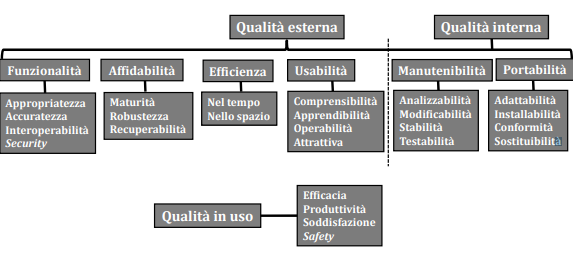
\includegraphics{images/gerarchiaQualitaProdotto.png}
		\caption{Riepilogo modello ISO 9126}
	\end{figure}